\documentclass{beamer}
\usetheme{Madrid}

\usepackage{amsmath, amssymb, amsthm}
\usepackage{graphicx}
\usepackage{listings}
\usepackage{gensymb}
\usepackage{minted}
\usemintedstyle{friendly}
\definecolor{bg}{rgb}{1.0, 1.0, 0.8}
\usepackage[utf8]{inputenc}
\usepackage{hyperref}
\usepackage{gvv}
\begin{document}
\title{MATRIX THEORY-MATGEO PRESENTATION}
\author{EE24BTECH11008 - ASLIN GARVASIS}
\date{}
\frame{\titlepage}

\begin{frame}
\frametitle{Question}
If $\vec{A}\brak{\frac{a}{3},4}$ is the midpoint of the line segment joining the points $\vec{B}\brak{-6,5}$ and $\vec{C}\brak{-2,3},$  
		then the value of $a$ is\\ \\
  \hfill{CBSE $\brak{10-2021}$}
  \end{frame}
  \begin{frame}{allowframebreaks}
\frametitle{Solution: Table}
\begin{table}[h!!]
    \centering
    \begin{tabular}{|c|c|}
\hline
\textbf{Variable}& \textbf{Description}
\\\hline
$\vec{B}$$\brak{-6,5}$ &  coordinates of first point\\
    \hline 
        $\vec{C}$$\brak{-2,3}$ & coordinates of second point\\
    \hline
        $\vec{A}$& midpoint of $\vec{B}$ and $\vec{C}$\\ 
    \hline
        $k$ & ratio in which $\vec{c}$ divides the line joining $AB$\\
    \hline
	$\frac{\vec{C}+k\vec{B}}{k+1}$ & section formula\\
    \hline
\end{tabular}
    \caption{Variables Used}
\end{table}
\end{frame}
\begin{frame}
\frametitle{Theory}
\begin{align}
 \vec{A} &=\frac{k\vec{C}+\vec{B}}{k+1}
\end{align}
\end{frame}
\begin{frame}{Theory}
    where k is the ratio which $\vec{A}$ divides $\vec{B}$ and $\vec{C}$,\quad here k=1 $\brak{\because \text{midpoint}}$\\
\end{frame}
\begin{frame}{Theory}
\begin{align}
\implies \vec{A}&=\frac{\vec{B}+\vec{C}}{2}\\ 
\implies \vec{A}&=\frac{\myvec{-6\\5}+\myvec{-2\\3}}{2}=\frac{\myvec{-8\\8}}{2}=\myvec{-4\\4}\\
\because \vec{A}&=\myvec{\frac{a}{3}\\4}\\
\implies a&=-4\times3\\ 
\implies a&=-12
\end{align}    
\end{frame}
\begin{frame}
\frametitle{Simulation}
\begin{figure}
    \centering
    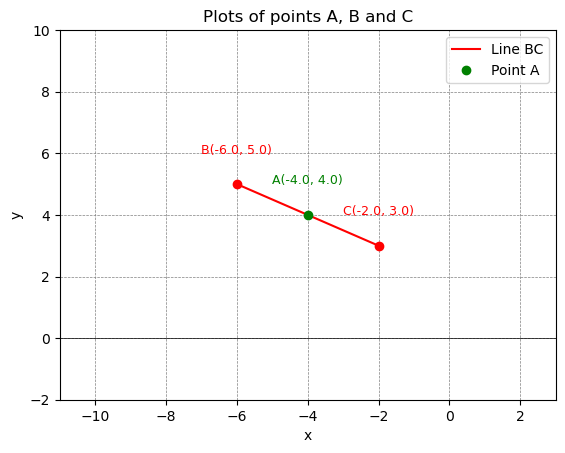
\includegraphics[width=0.7\linewidth]{plot.png}
\end{figure}
\end{frame}
\begin{frame}[fragile]
\frametitle{C-code}
\begin{minted}[bgcolor=bg, linenos, fontsize=\small, breaklines]{c}
    #include <stdio.h>

int main() {
    FILE *file = fopen("points.txt", "w");
    if (file == NULL) {
        printf("Error opening file!\n");
        return 1;
    }

    // Define the points
    int x1 = -6, y1 = 5;
    int x2 = -2, y2 = 3;
 \end{minted}   
 \end{frame}
 \begin{frame}[fragile]
 \frametitle{C-code}
   \begin{minted}[bgcolor=bg, linenos, fontsize=\small, breaklines]{c}  
    fprintf(file, "Point 1: (%d, %d)\n", x1, y1);
    fprintf(file, "Point 2: (%d, %d)\n", x2, y2);

    // Close the file
    fclose(file);

    return 0;
}
\end{minted}
\end{frame}
\begin{frame}{Output in points.txt}
\begin{center}
    Point \quad$1: \brak{-6, 5}$\\
    Point \quad$2: \brak{-2, 3}$
\end{center}
\end{frame}
\begin{frame}[fragile]
\frametitle{Python code}
    \begin{minted}[bgcolor=bg, linenos, fontsize=\small, breaklines]{python}
import sys               
#for path to external scripts
sys.path.insert(0, '/home/matgeo/codes/CoordGeo')
#path to my scripts

import numpy as np
import numpy.linalg as LA
import matplotlib.pyplot as plt
import matplotlib.image as mpimg

#local imports
from line.funcs import *
\end{minted}
\end{frame}
\begin{frame}[fragile]
\frametitle{Python code}
\begin{minted}[bgcolor=bg, linenos, fontsize=\small, breaklines]{python}
# Read the points from the file
with open('points.txt', 'r') as file:
    lines = file.readlines()

# Extract the coordinates
point1_str = lines[0].strip().split(': ')[1]  
# Get the string after 'Point 1 : '
point2_str = lines[1].strip().split(': ')[1]  
# Get the string after 'Point 2 : '

# Convert the string coordinates to tuples
# Use eval to convert string to tuple
x1, y1 = eval(point1_str)  
x2, y2 = eval(point2_str)
\end{minted}
\end{frame}
\begin{frame}[fragile]
\frametitle{Python code}
\begin{minted}[bgcolor=bg, linenos, fontsize=\small, breaklines]{python}
B=np.array([x1,y1]).reshape(-1,1)
C=np.array([x2,y2]).reshape(-1,1)
A=np.array([(x1+x2)/2,(y1+y2)/2]).reshape(-1,1)
# generation of line
x_BC = line_gen(B,C)
# plotting line
plt.plot(x_BC[0,:],x_BC[1,:],label='$BC$')
#Labeling the coordinates
colors = np.arange(1,4)
tri_coords = np.block([[A,B,C]])
plt.scatter(tri_coords[0,:], tri_coords[1,:], c=colors)
vert_labels = ['A','B','C']
\end{minted}
\end{frame}
\begin{frame}[fragile]
\frametitle{Python code}
\begin{minted}[bgcolor=bg, linenos, fontsize=\small, breaklines]{python}
for i, txt in enumerate(vert_labels):
#plt.annotate(txt, # this is the text
    plt.annotate(f'{txt}\n({tri_coords[0,i]:.2f},{tri_coords[1,i]:.2f})',
            (tri_coords[0,i], tri_coords[1,i]), 
            # this is the point to label
            textcoords="offset points", 
            # how to position the text
            xytext=(25,5), 
            # distance from text to points (x,y)
            ha='center') 
            # horizontal alignment can be left, right or center

\end{minted}
\end{frame}
\begin{frame}[fragile]
\frametitle{Python code}
\begin{minted}[bgcolor=bg, linenos, fontsize=\small, breaklines]{python}
# use set_position
ax = plt.gca()
ax.spines['top'].set_color('none')
ax.spines['left'].set_position('zero')
ax.spines['right'].set_color('none')
ax.spines['bottom'].set_position('zero')
'''
ax.spines['left'].set_visible(False)
ax.spines['right'].set_visible(False)
ax.spines['top'].set_visible(False)
ax.spines['bottom'].set_visible(False)
plt.xlabel('$x$')
plt.ylabel('$y$')
plt.legend(loc='best')
'''
plt.grid()
plt.axis('equal')
plt.show()
\end{minted}
\end{frame}
\end{document}
